\documentclass[letterpaper,10pt,draftclsnofoot,onecolumn,titlepage]{IEEEtran}

\usepackage{graphicx}
\usepackage{amssymb}
\usepackage{amsmath}
\usepackage{amsthm}
\usepackage{alltt}
\usepackage{float}
\usepackage{color}
\usepackage{url}
\usepackage{enumitem}
\usepackage{pstricks, pst-node}
\usepackage{geometry}
\usepackage{array}
\usepackage{listings}
\usepackage{caption}
\usepackage{subcaption}


\geometry{margin = .75in}

\usepackage{hyperref}

\graphicspath{{figures/}{pictures/}{images/}{./}}


\newcommand*{\signature}[1]{%
	\par\noindent\makebox[3.5in]{\hrulefill} \hfill\makebox[3.0in]{\hrulefill}%
	\par\noindent\makebox[3.5in][l]{#1}	    \hfill\makebox[3.0in][l]{Date}%
}%

\def\name{Kevin Stine, Courtney Bonn, Maxwell Dimm}
\def\team{Calvary Chapel Corvallis}
\def\grp{Group \#62}

\hypersetup{
	colorlinks = true,
	urlcolor = black,
	linkcolor = black,
	pdfauthor = {\name},
	pdftitle = {CS463 Progress Report},
	pdfsubject = {CS463 Progress Report},
	pdfpagemode = UseNone
}

\begin{document}
	\title{\huge \team \\ Progress Report\\ CS 463 Spring 2017}
	\author{\large \name \\ \grp}



	\maketitle

		\begin{abstract}The purpose of this project is to produce an iOS/Android application for Calvary Chapel of Corvallis that will allow members to access a plethora of information all in one localized space.
		The Church's current website does not provide an interface where current members of the church can very quickly access important information such as events, bulletins, and messages from the service.
		The desired application will be simple enough for anyone to use while providing back end access for staff to easily upload new information to the app.
		The priorities lie in maximizing the usability of the app and providing bulletin, schedule, video, and giving functionality.
		We will work with the existing Calvary Chapel web development team to create a product that is seamlessly integrated with their already existing network.
		\end{abstract}

		\clearpage

\section{Purpose and Goals}
		The purpose of our project is to create an application for Calvary Corvallis Church that will act as a connection between the congregation and the administration.
		The church already has a website that has some of this information, but they want the website and app to serve different functions.
		The website will be to introduce people to the church.
		The app will be used for the existing congregation as the go to place to access the most commonly used or needed information.
		Some of the features being provided within the app are: having sermons available, listing the bulletin, having the church schedule, and allowing members to donate to the church.
		Our client explained to us that these were the features that they wanted in the app as they are the most needed services by their members.

		Our client has requested that the app be as automated as possible in regards to updating the information hosted within it as to reduce any upkeep as much as possible.
		So we will be working with their existing infrastructure as much as possible to pull our information from.
		We are also creating both an iOS and Android application and we want to make the applications as functionally similar as possible.
		This will allow for greater understanding of the app across users who may or may not be super tech savvy.
		Our final goal in this project is to reduce costs wherever possible for our client.
		If that means suggesting newer cheaper infrastructure or setting up our app in a way that reduces how often it will need to be updated, we want to do it.

\section{Fall 2016}
		During the first few months of working with this project, we focused on learning what our client wanted, determining the exact requirements, designing the projects, and learning how to develop mobile applications.
		 Though no implementation took place during this time, a large bulk of the design decisions and specifics about the applications were completed which set us up for a smooth transition into development.
		The requirements of the project were decided between us and the client.
		The main requirements included a bulletin page, a calendar, the ability to donate, and the ability to watch the most recent sermon.
		Additionally, the client wanted a simple interface that looked similar to their current website and was not cluttered with too much information.
		Other requirements included having the application available on both iOS and Android smart phones and working with their existing back end software and website.

		To meet the requirement of having the app available on multiple platforms, we decided to create two native applications using Xcode and Android Studio.
		We used the incorporated Interface Builder to design the iOS app and we used a navigation drawer system in Android Studio.
		The bulletin page was originally going to work with their back end software, Church Community Builder, but after the church changed their current website to Wordpress, we were able to pull directly from their website page.
		The events are being extracted from Church Community Builder and the messages page is working with LiveStream.


\section{Winter 2017}
		Most of the implementation of the iOS implementation was done during Winter term.
		The first couple weeks were spent continuing to learn how Xcode and Android Studio worked and getting our base applications up and running.
		Once we grasped the basic development concepts, we began working on our individual pieces.
		Originally, the project was divided the following way:
		\begin {itemize}
			\item Bulletin Page and iOS Interface: Courtney
			\item Events Page and Android Interface: Kevin
			\item Messages and Donations: Max
		\end {itemize}
		However, assignments were shifted when individual pieces were more difficult than we originally thought.
		Throughout the development process, the project shifted in the following way:
		\begin {itemize}
			\item Bulletin Page, Events Page (Android), Donation Page (Android): Courtney
			\item Events Page (iOS): Kevin
			\item Donation Page (iOS), Messages Page: Max
		\end {itemize}

		We discovered that the Events page was more involved than we planned for and ended up needing to split the responsibilities in order to have this page finished on time.
		The specifics of each page will be described below.


		By the end of Winter term, we had two almost completed applications.
		We focused on the iOS implementation because that was the one we began first and spent the most time on.
		The iOS app had the home page, bulletin page, donation page, and most of the messages page finished at this point.
		The events page was still being worked on but it was in progress.

		The Android implementation was slower to begin and was about halfway done at the end of this term.
		Only the bulletin and the donation pages were finished by this point.



\section{Current Status}
		Beginning Spring term, we still had quite a bit of work to finish before the apps were completed.
		Though the goal was to finish development by Winter term, this did not happen.
		We focused on finishing the Android app as it had the furthest to go before being done.
		At the same time, we did continue to work on the iOS app to try and get them both complete as soon as possible.

		As of now, both apps are finished, though neither are available for download in their respective stores.
		The client has decided to continue working on the app and adding additional information, which is discussed below, and they want to hold off on publishing the applications.
		However, our original requirements have been met with the apps as they are.

		On the iOS app, an XML Parser was used to request and parse the public calendar from Church Community Builder.
		The parsed information was then presented in a UITableView.
		When a user clicks on each event, they can see an additional view with more details, like time, location, group leader, and contact information.
		Here is a code snippet from the iOS version of the EventViewController:

		\begin{lstlisting}
func createDatePicker() {
    // format the picker
    datePicker.datePickerMode = UIDatePickerMode.date
    //toolbar
    let toolbar = UIToolbar()
    toolbar.sizeToFit()
    // bar button item
    let doneButton = UIBarButtonItem(barButtonSystemItem:
			.done, target: nil, action: #selector(donePressed))
    toolbar.setItems([doneButton], animated: false)
    changeDate.inputAccessoryView = toolbar
    changeDate.inputView = datePicker
}
		\end{lstlisting}
		This code creates the datePicker which allows the user to select the month, day and year.
		While the day function does not work (per our client's request), it does allow the user to select the month and year.
		This sets up the date picker using the UiDatePicker, and adds a UIToolbar to the top which allows the user to cancel picking the date,
		or pass the selected date to be set as the end URL.

		\begin{lstlisting}
func donePressed() {
    // format date
    let dateFormatter = DateFormatter()
    dateFormatter.dateFormat = "yyyy-MM-dd"
    pickerTracker = true
    startDate = dateFormatter.string(from: datePicker.date)
    updateTable()
    self.view.endEditing(true)
}
		\end{lstlisting}

		This code is the selected action for the DatePicker.
		When the user pressed done, the selector is set and will call the donePressed function which sets the new start date to the one the user selects.
		\par
		The Android app is very similar, though with the language difference, a new XML Parser was needed.
		Again the information is requested and parsed from the public calendar, and then presented in a List View.
		Users are also able to click on each event and view additional details.
		A code snippet from the XML Parser is listed below:

		\begin{lstlisting}
 public String getXmlFromUrl(String url) {
       OkHttpClient client = new OkHttpClient();
           final String basic = "Basic " + Base64.encodeToString(CREDENTIALS.getBytes(),
           Base64.NO_WRAP);
           String str = null;
           Request request = new Request.Builder()
                   .url(url)
                   .header("Authorization", basic)
                   .build();

           try {
               Response response = client.newCall(request).execute();
               str = response.body().string();
           } catch (IOException e) {
               e.printStackTrace();
           }

       return str;
   }
   		\end{lstlisting}

		We used OkHttpClient in order to request the XML response from the URL.
		Once we received the response, we parsed it using a Document Builder Factory.
		The end results on how this response is displayed on the app can be seen in Figure ~\ref{fig:event}.

		\begin{figure}[H]
			\centering
			\begin{subfigure}{.5\textwidth}
 				 \centering
  				 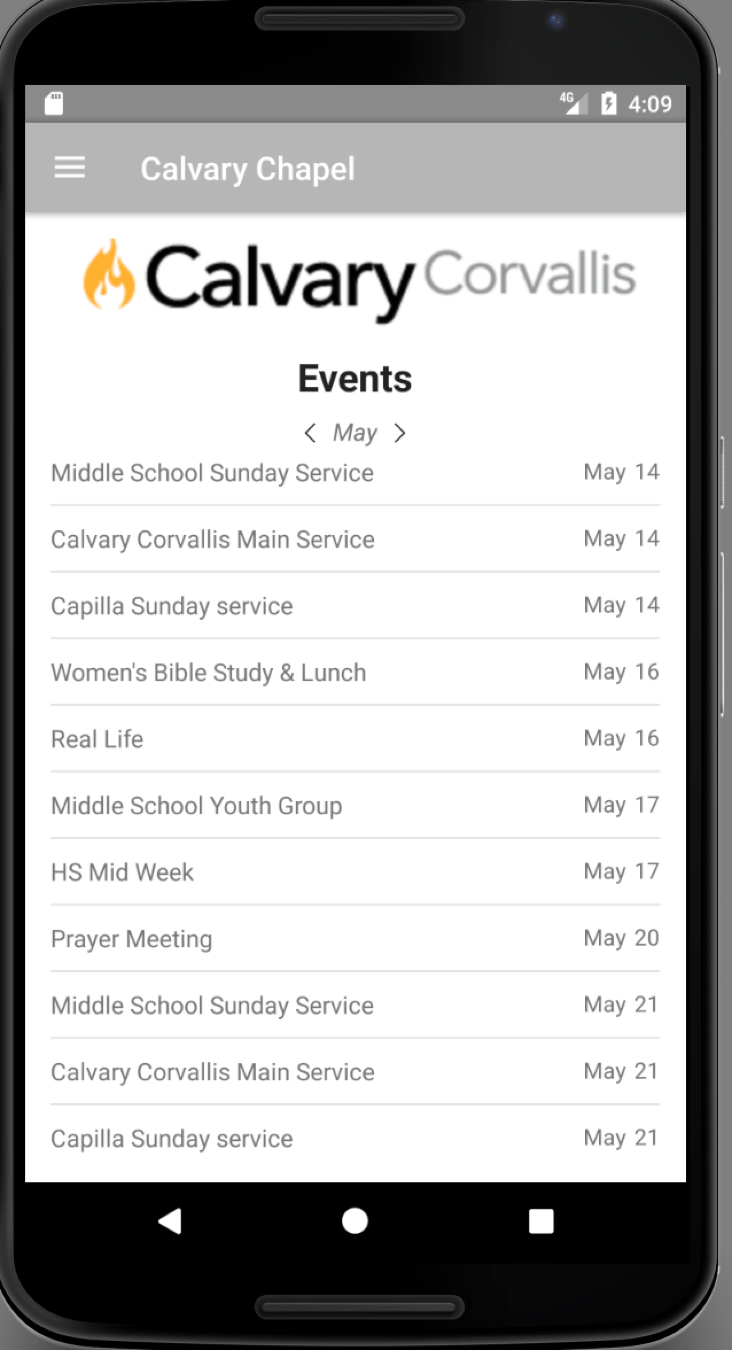
\includegraphics[width=.4\linewidth]{androidevents}
 				 \caption{A List of Events}
  				 \label{fig:sub1}
			\end{subfigure}%
			\begin{subfigure}{.5\textwidth}
		         	\centering
 				 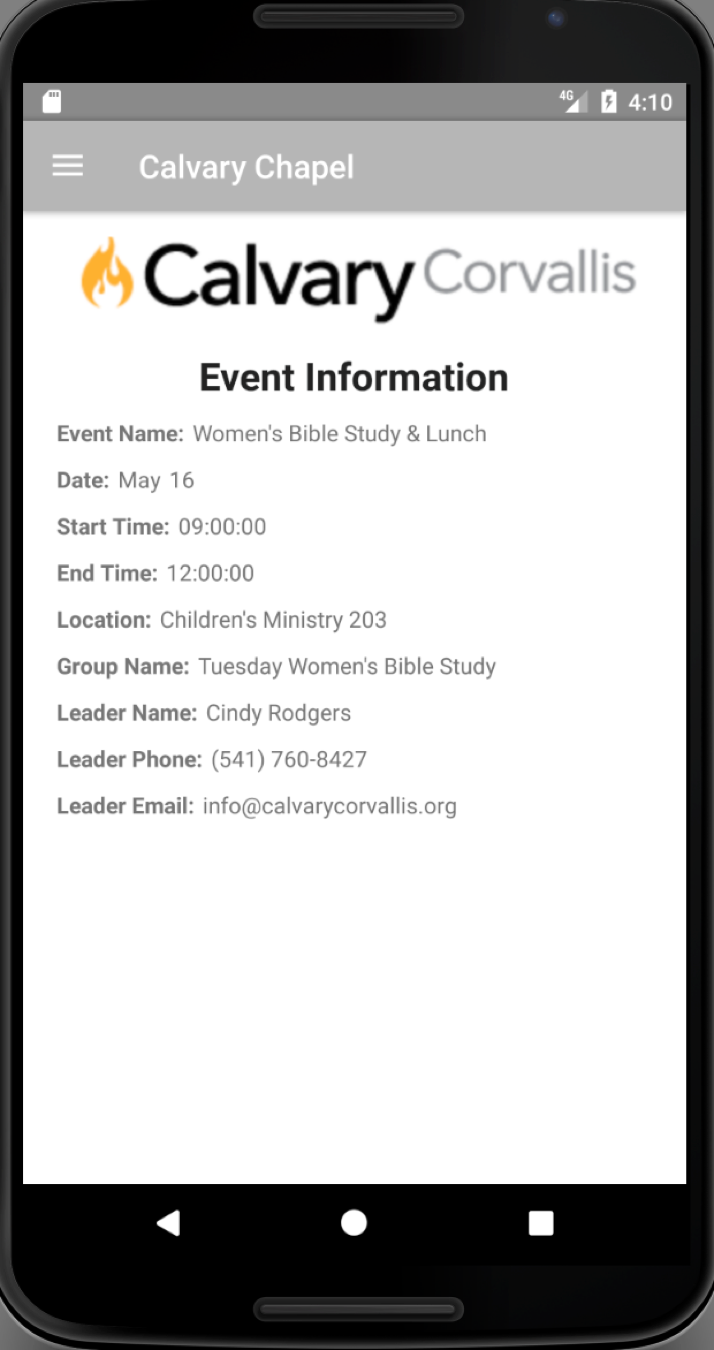
\includegraphics[width=.4\linewidth]{androiddetails}
 				 \caption{An Event Details}
 				 \label{fig:sub2}
			\end{subfigure}
			\caption{Android Event Page}
			\label{fig:event}
		\end{figure}

		The Bulletin page is an exact replica of the corresponding page on Calvary's website on both the iOS and Android app.
		The church was in the process of creating a new website that was powered by Wordpress.
		Wordpress sites can be parsed using JSON and REST API.
		The response from the request is a JSON Object that can be parsed and information can be pulled from the response.
		A JSON Parser was used to request the bulletin page on the website and the response we received was the content of the page.
		A sample response from the JSON request was:

		\begin{lstlisting}

{
  "id": 1038,
  "date": "2016-10-27T19:22:53",
  "date_gmt": "2016-10-27T19:22:53",
  "guid": {
    "rendered": "http://www.calvarycorvallis.org/?page_id=1038"
  },
  "modified": "2017-03-18T11:48:50",
  "modified_gmt": "2017-03-18T18:48:50",
  "slug": "bulletin",
  "status": "publish",
  "type": "page",
  "link": "https://www.calvarycorvallis.org/bulletin/",
  "title": {
    "rendered": "This Week&#8217;s Bulletin"
  },
  "content": {
    "rendered": "<p>all bulletin content would be here...
    ...
    },
    Additional, unrelated JSON returned below here...
 }



		\end{lstlisting}

		From this response, the "content": \{ "rendered": .. \} was the part that contained that actual bulletin content that would need to be displayed on the application.
		The parsing for iOS is listed below:

		\begin{lstlisting}
 do {
 	guard let bulletin = try JSONSerialization.jsonObject(with: responseData,
	options: []) as? [String: AnyObject] else {
	         print("error trying to convert data to JSON")
                 return
         }

        	guard let bulletinContent = bulletin["content"]?["rendered"] as?
	String else {
                  print("Could not get bulletin content from JSON")
                  return
         }
         let actualContent = bulletinContent.replacingOccurrences(of: "<[^>]*.", with:
         "", options: .regularExpression, range: nil)

         DispatchQueue.main.async{
 	          self.jsontext.text = actualContent
         }
} catch  {
         print("error trying to convert data to JSON")
         return
}
\end{lstlisting}

		The parsing for Android, which was simpler to extract the needed information is below:

		\begin{lstlisting}
if (response != null) {
	try {
		JSONObject jsonResponse = response.getJSONObject(TAG_CONTENT);
                 String jsonData = jsonResponse.getString(TAG_RENDERED);
		 textView.setText(jsonData);
                  Log.e("App", "Success: " + response.getString("yourJsonElement"));
	} catch (JSONException ex) {
                    Log.e("App", "Failure", ex);
        }
}
	\end{lstlisting}


		In order to style the content similarly to the way the website is styled, the response was wrapped in HTML and CSS and loaded into a Web View.
		This was done slightly differently but very similarly within each app.

		For iOS, loading into a UIWebView was as follows:
		\begin{lstlisting}
let htmlCode = "<!DOCTYPE HTML><html><head><style> body {color: #5b5e5e; font-family:
'Lora', Palatino;} a { border-bottom: 1px solid #fbaf17; color: #fbaf17;
text-decoration: none; }
.staff a { border-bottom: 0px none; } a:focus, a:hover { border-bottom: 1px solid #fbaf17;
color: #b17b0e; }</style></head><body>" + bulletinContent + "</body></html>"

self.bulletinWeb.loadHTMLString(htmlCode, baseURL: nil)
		\end{lstlisting}

		For Android, loading into a Web View is listed below:
		\begin{lstlisting}
String bulletinContent = "<!DOCTYPE HTML><html><head><style> body {color: #5b5e5e;
font-family: 'Lora', Palatino;} a { border-bottom: 1px solid #fbaf17; color: #fbaf17;
text-decoration: none; } .staff a { border-bottom: 0px none; } a:focus, a:hover {
border-bottom: 1px solid #fbaf17; color: #b17b0e; }</style></head><body>" +
jsonData + "</body></html>";

myWebView.loadDataWithBaseURL("file:///android_asset/", bulletinContent,
"text/html", "utf-8", null);
myWebView.getSettings().setAllowFileAccess(true);
		\end{lstlisting}

		With the above listed code, the bulletin page was rendered on the app and styled to look almost exactly as it does on the website.
		The resulting bulletin page on both devices can be seen in Figure ~\ref{fig:bulletin}.

		\begin{figure}[H]
			\centering
			\begin{subfigure}{.5\textwidth}
 				 \centering
  				 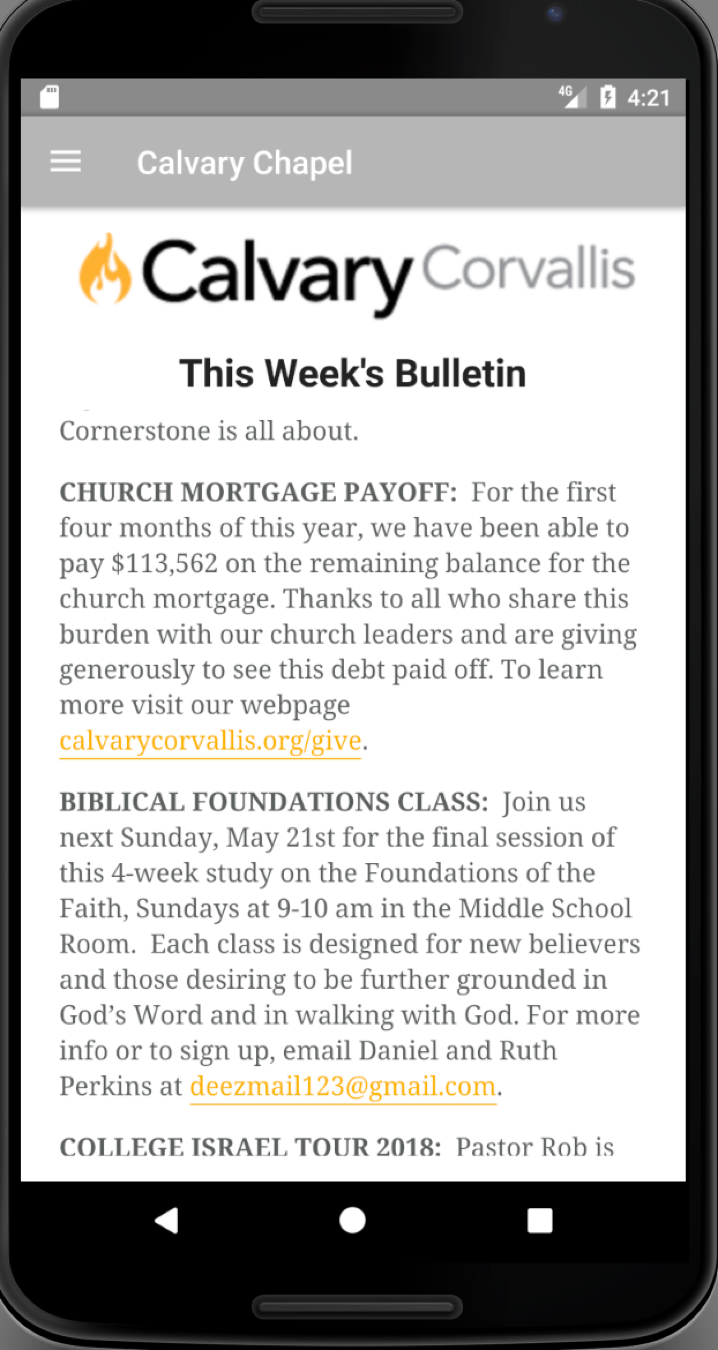
\includegraphics[width=.4\linewidth]{androidbulletin}
 				 \caption{Android}
  				 \label{fig:sub1}
			\end{subfigure}%
			\begin{subfigure}{.5\textwidth}
		         	\centering
 				 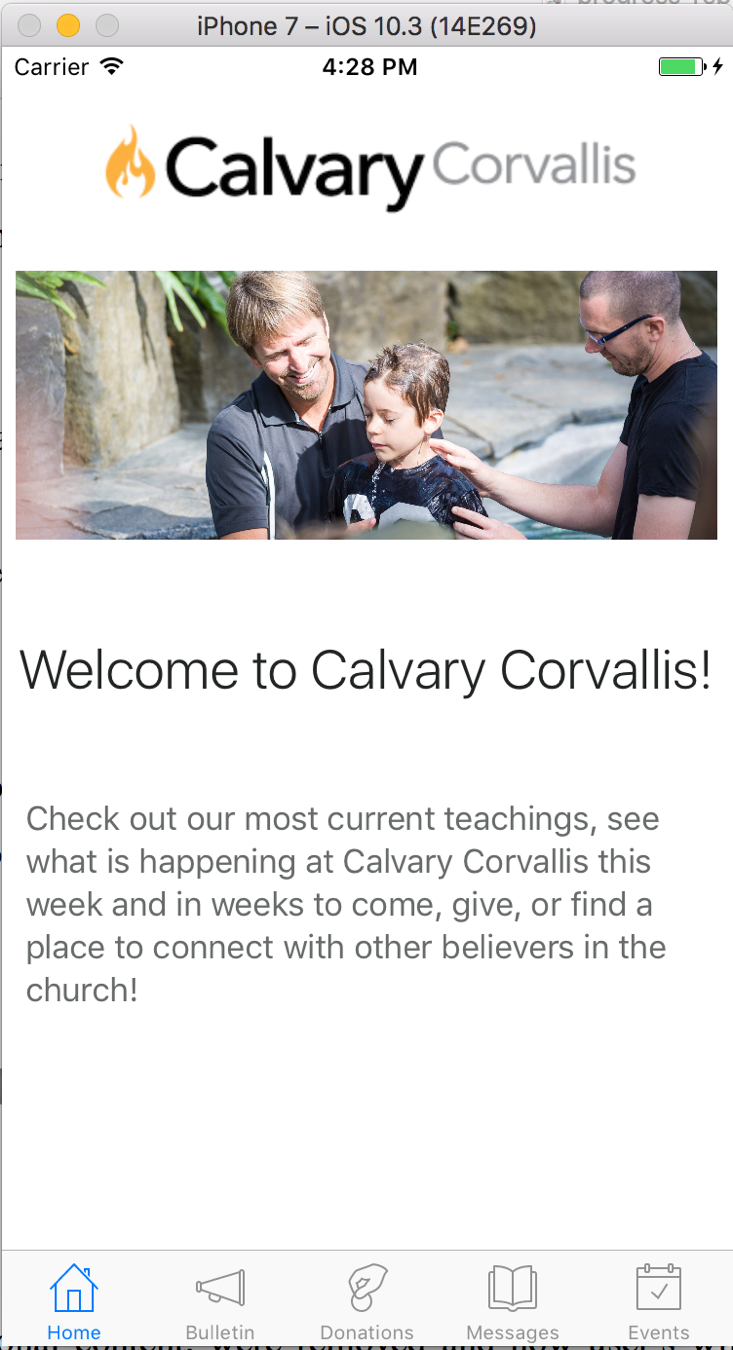
\includegraphics[width=.4\linewidth]{iosbulletin}
 				 \caption{iOS}
 				 \label{fig:sub2}
			\end{subfigure}
			\caption{Bulletin Page}
			\label{fig:bulletin}
		\end{figure}




		Because the Donation page handles sensitive information, we decided with our client not to have the application handle the private information.
		Instead, the entire donation page was loaded into a UIWebView from the Calvary website.
		The header, footer, and additional content, were removed and now user's will have the ability to donate quickly while still protecting their credit card and personal information.

		On the iOS app, the code that was used to load this page is listed below:
		--ios code here


		The code for handling the loading of this page for Android is listed below:
		\begin{lstlisting}
@Override
    public void onPageFinished(WebView view, String url) {
            myWebView.loadUrl("javascript:(function() { " +
            "document.getElementsByClassName('site-header')[0].style.display='none'; " +
            "document.getElementsByClassName('footer-widgets')[0].style.display='none'; " +
            "document.getElementsByClassName('content')[0].style.display='none'; " + "})()");
            myWebView.setVisibility(View.VISIBLE);
            myWebView.getSettings().setLoadWithOverviewMode(true);
            myWebView.getSettings().setUseWideViewPort(true);
   	}
   });
        myWebView.setVisibility(View.GONE);
        myWebView.loadUrl("https://www.calvarycorvallis.org/give/");
        		\end{lstlisting}

		The donation page on both devices can be seen in Figure ~\ref{fig:donation}.

		\begin{figure}[H]
			\centering
			\begin{subfigure}{.5\textwidth}
 				 \centering
  				 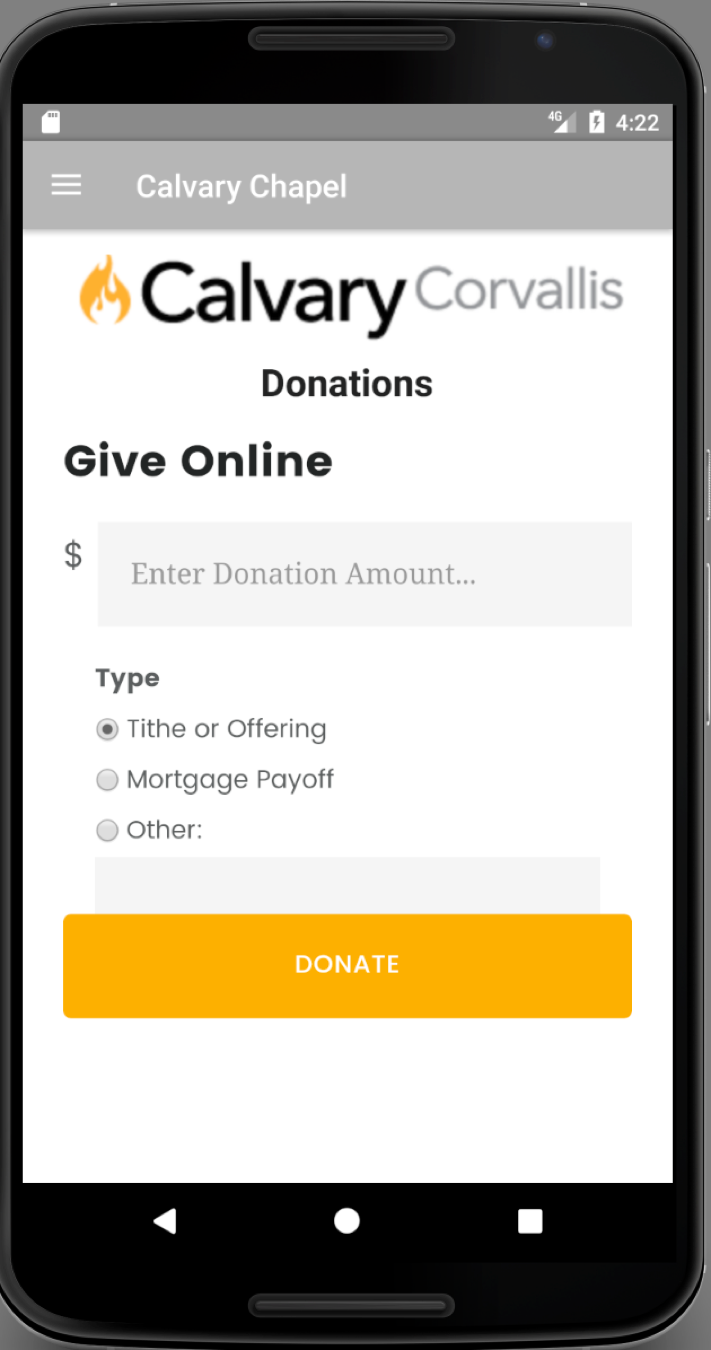
\includegraphics[width=.4\linewidth]{androiddonate}
 				 \caption{Android}
  				 \label{fig:sub1}
			\end{subfigure}%
			\begin{subfigure}{.5\textwidth}
		         	\centering
 				 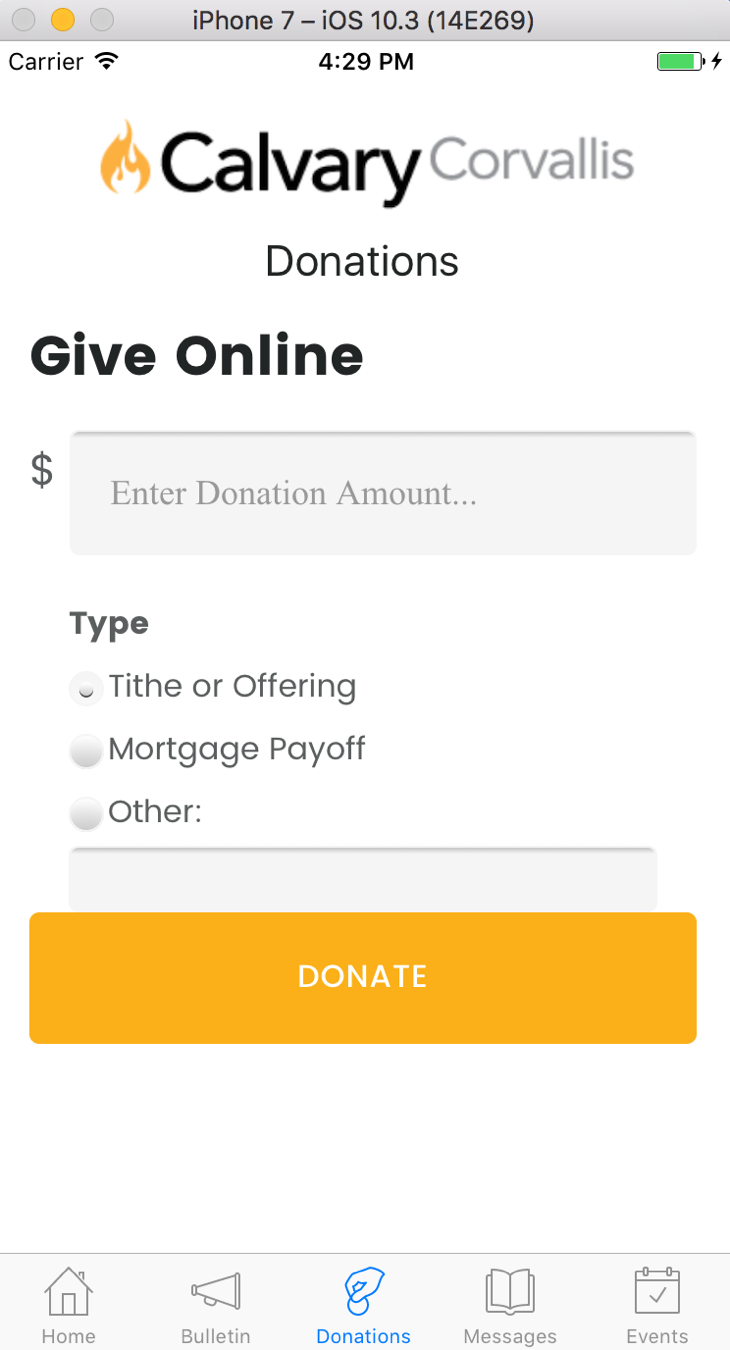
\includegraphics[width=.4\linewidth]{iosdonate}
 				 \caption{iOS}
 				 \label{fig:sub2}
			\end{subfigure}
			\caption{Donation Page}
			\label{fig:donation}
		\end{figure}


		The messages page is a hard coded video from Calvary's LiveStream account, along with a button to access previous videos.
		Issues with the client's LiveStream account will be discussed further below, but they did cause this page to not be exactly what we need.

		The messages page on both devices can be seen in Figure ~\ref{fig:message}.

		\begin{figure}[H]
			\centering
			\begin{subfigure}{.5\textwidth}
 				 \centering
  				 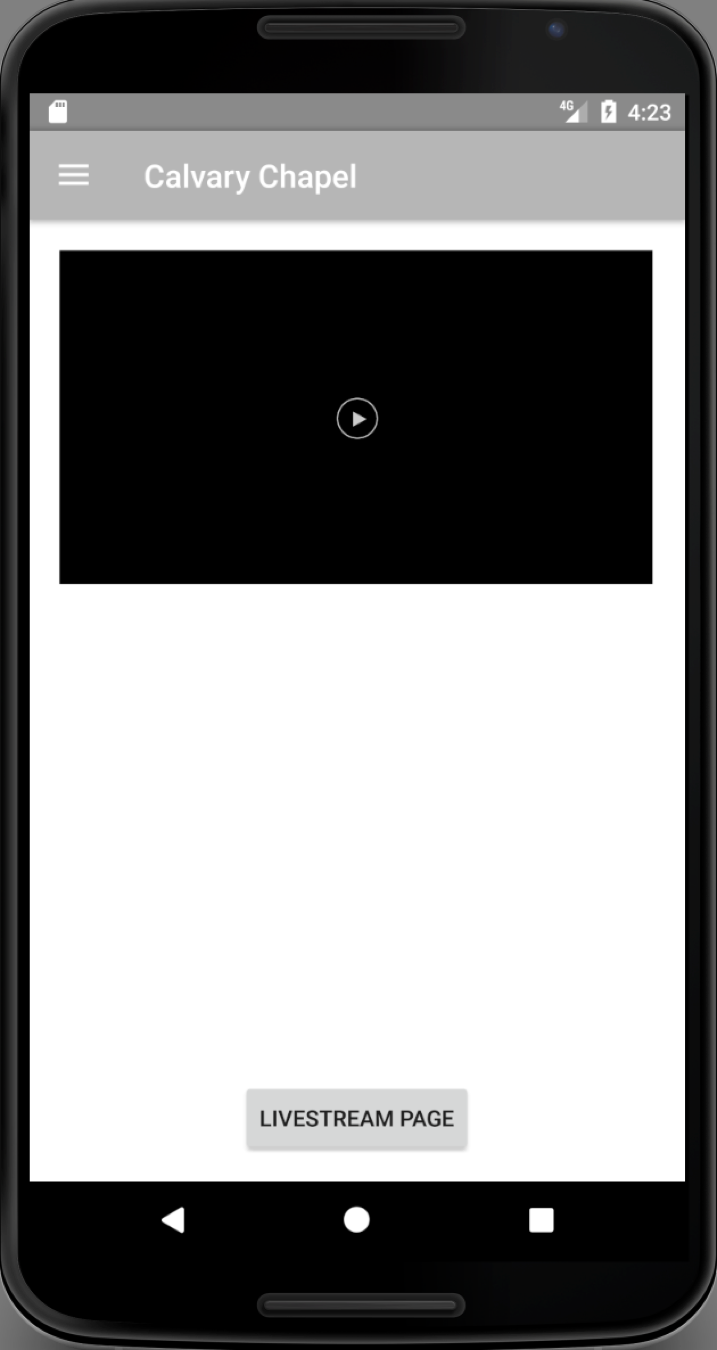
\includegraphics[width=.4\linewidth]{androidmessages}
 				 \caption{Android}
  				 \label{fig:sub1}
			\end{subfigure}%
			\begin{subfigure}{.5\textwidth}
		         	\centering
 				 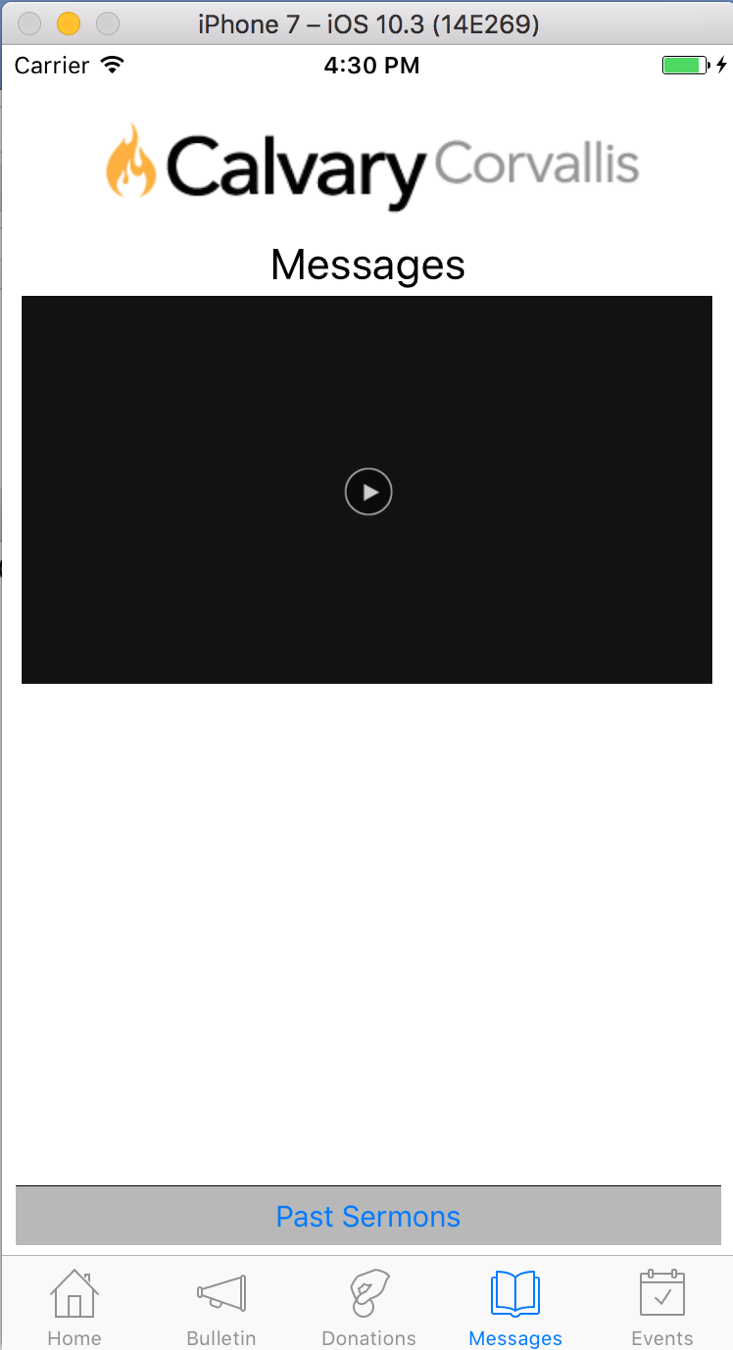
\includegraphics[width=.4\linewidth]{iosmessages}
 				 \caption{iOS}
 				 \label{fig:sub2}
			\end{subfigure}
			\caption{Messages Page}
			\label{fig:message}
		\end{figure}


\section{Problems Encountered}

\section{Future Work}
		Within the last few weeks, the client has realized there are additional features they would like to be present on the applications.
		Because of time constraints, we were not able to complete these features for the client.
		However, the client does have a web development team that we will be turning the project over to and they will continue to develop and add to what we have developed.

		The additional features include push notifications, multiple languages, the ability to fill out registration forms for events, and possible additional pages.

		For the push notifications, the client wants to be able to alert their members when there is an event cancelled, such as a church service, or other emergency alerts.
		At this time, we are unable to implement push notifications.
		On the iOS app, notifications require a developer account to be able to implement and test.
		Our client does have a developer account and will have the ability to add notifications.
		On the Android app, notifications are sent out through Google Cloud Messaging which would add an additional service the church would need to keep track of.
		Our client has not decided whether or not they would want to add this service, so notifications will not be implemented on the Android app right now.

		About halfway through development, the client wondered about the possibility of making the app available in different languages.
		Because this was not part of the original requirements, we set it as a stretch goal to complete if we had finished all other requirements and still had time to spare.
		As of this time, we were not able to implement this for the client as the original requirements took longer to complete.

		Recently, the client wanted to add the ability to fill out registration forms for particular events.
		The theory would be that a person could click on an event, see a registration link, and fill out the form directly on the app and submit it to the church.
		Currently, we are trying to test this function with test events and are waiting for the client to add a test form.
		More than likely we will not be able to finish this implementation before we are finished with the project.

		The client's senior staff has ideas of future pages or content that could be added to the app.
		Adding pages to the apps is a relatively easy task and will be explained to the development team when we are finished with the project.
		They are not sure what kind of content may be added, but they want to keep the possibility of more pages open.








\end{document}
